\chapter{Data Flows}
\label{ch:data-flows}

\section{Principal data flow: generation}

\begin{figure}[H]
\centering
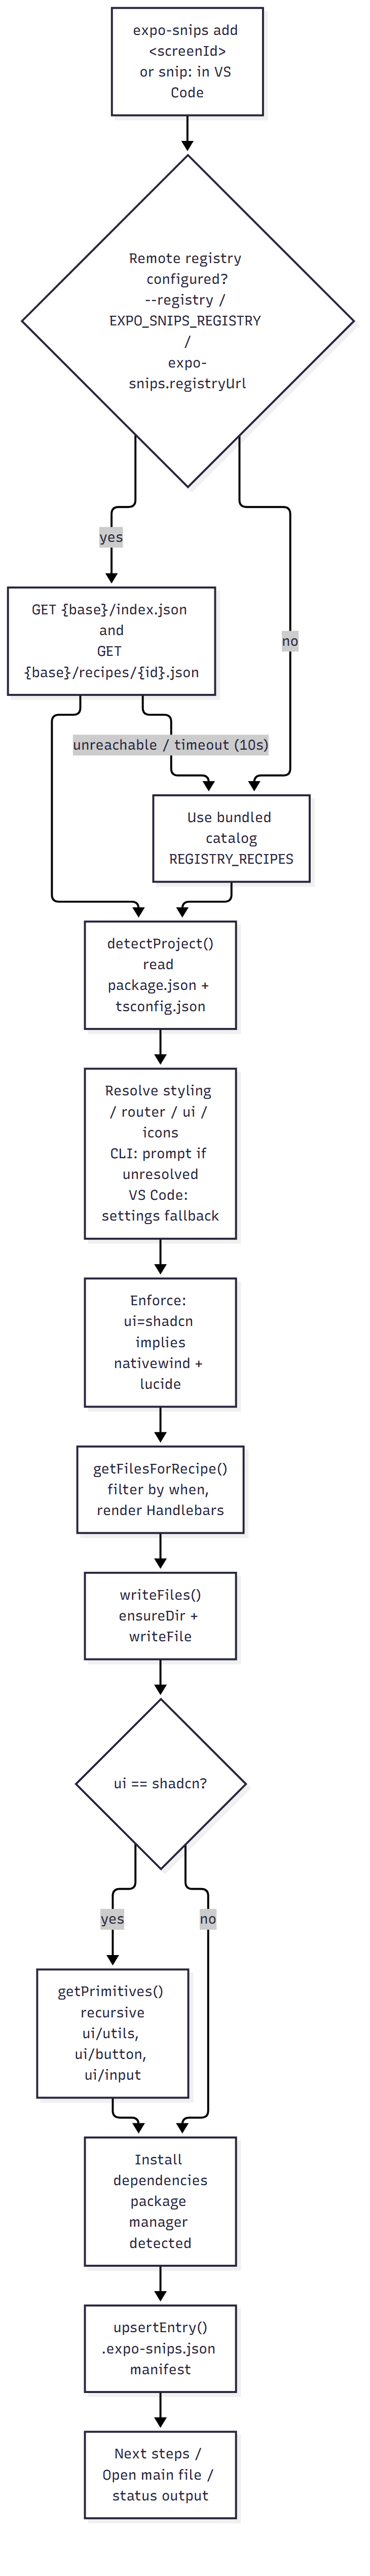
\includegraphics[width=\textwidth]{diagrams/generation-pipeline.png}
\caption{Generation data flow: from command input to persisted manifest}
\label{fig:data-flow-generation}
\end{figure}

\subsection*{Data transformations}

\begin{longtable}{p{3.4cm}p{4.4cm}p{6.6cm}}
\caption{Data transformations in the generation flow}\\
\toprule
\textbf{Input} & \textbf{Transformation} & \textbf{Output} \\
\midrule

Registry base string & \texttt{trim()} then strip trailing \texttt{/} & Normalised base \\
Index JSON array & Map to \texttt{RecipeIndexEntry[]} & Browsable index \\
Recipe JSON & Object with \texttt{files[].template} strings & \texttt{ScreenRecipe} \\
\texttt{package.json} + \texttt{tsconfig.json} & Four dependency probes + one file
probe & \texttt{DetectedProject} \\
Flags + detection + recipe \texttt{supported} & Precedence rules, prompts,
shadcn enforcement & \texttt{GenerationOptions} \\
\texttt{GenerationOptions} + variant & \texttt{buildRenderContext} & \texttt{RenderContext} \\
Recipe + context & \texttt{when} filter, template selection, Handlebars compile and
execute & \texttt{\{path, content\}[]} \\
File list + project root & \texttt{ensureDir} + \texttt{writeFile} & Files on disk \\
Recipe metadata & \texttt{upsertEntry} & Manifest entry \\
\bottomrule
\end{longtable}

\section{Registry resolution flow}

\begin{figure}[H]
\centering
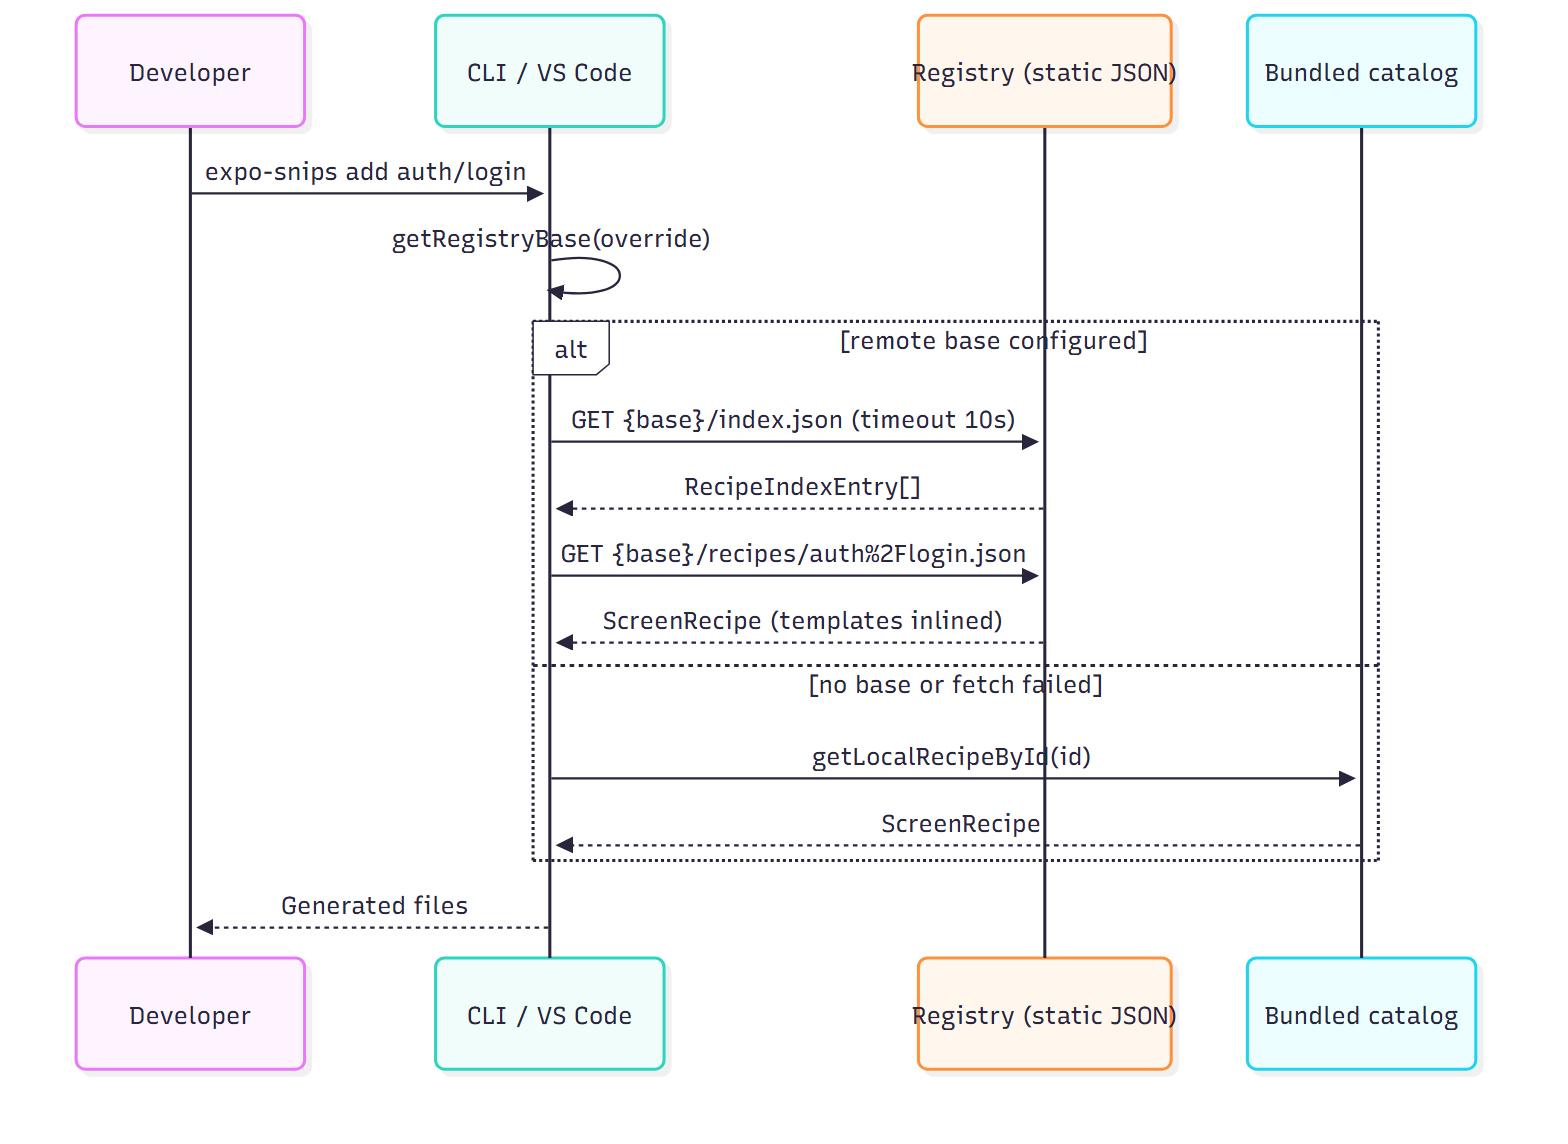
\includegraphics[width=0.94\textwidth]{diagrams/registry-api-sequence.png}
\caption{Sequence for resolving a recipe, including fallback}
\label{fig:data-flow-registry}
\end{figure}

\section{Primitive resolution flow}

\begin{figure}[H]
\centering
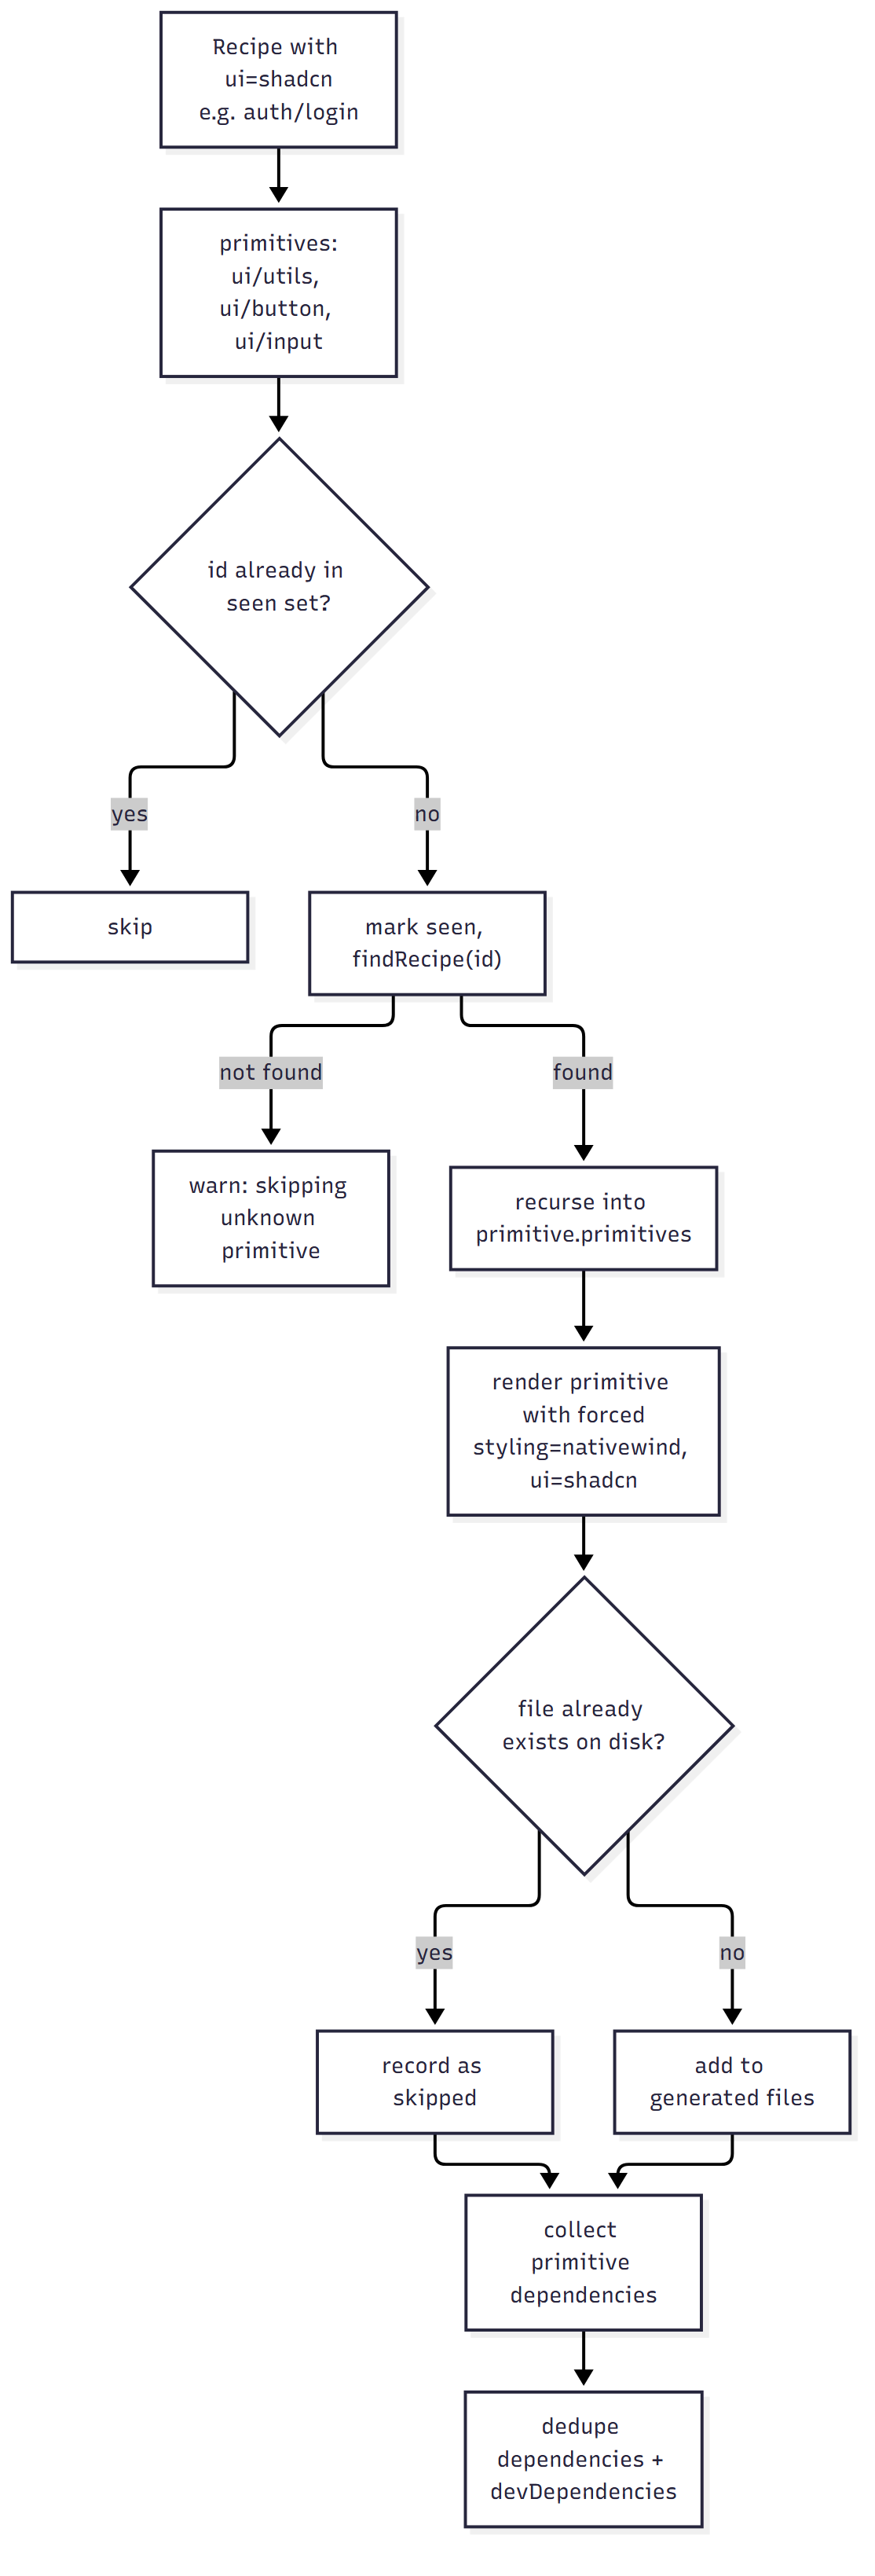
\includegraphics[width=0.95\textwidth]{diagrams/primitive-resolution.png}
\caption{Recursive primitive resolution data flow}
\label{fig:data-flow-primitives}
\end{figure}

The recursion is the only graph traversal in the codebase. It is guarded by a
\texttt{Set<string>} of seen ids, which makes the traversal terminate even if a
primitive cycle were introduced. Files whose paths already exist are excluded from
the generated set and reported as skipped.

\section{Update flow}

\begin{figure}[H]
\centering
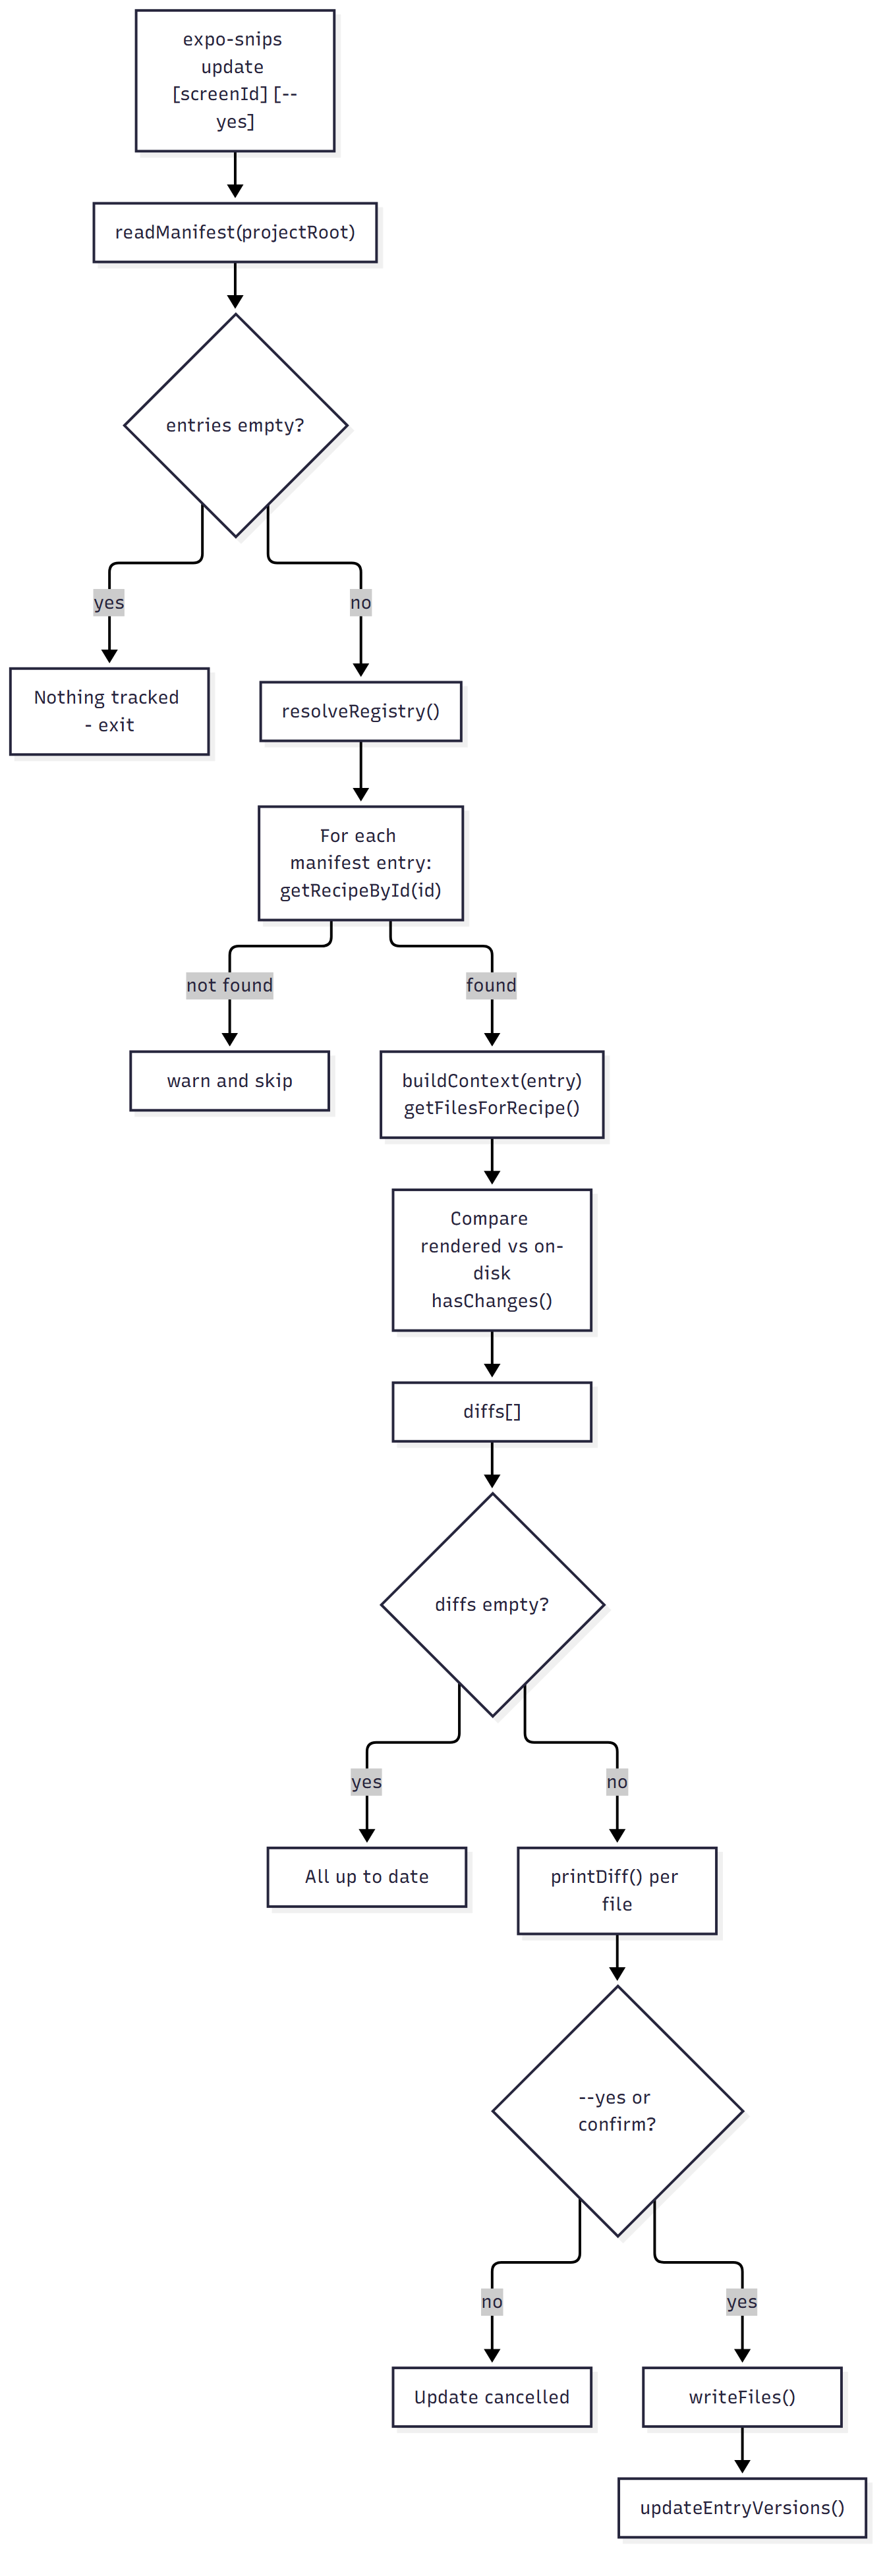
\includegraphics[width=0.95\textwidth]{diagrams/update-flow.png}
\caption{Update flow with diff preview and confirmation}
\label{fig:update-flow}
\end{figure}

\subsection*{Diff data structure}

\begin{lstlisting}[language=JavaScript]
interface DiffHunk { type: "add" | "remove" | "context"; line: string; }
\end{lstlisting}

\texttt{diffLines} builds an $(n+1) \times (m+1)$ dynamic-programming table over the
two line arrays (where $n$ and $m$ are the line counts) and walks it to emit hunks.
The algorithm is the classic longest-common-subsequence diff; it has no
line-number tracking, no hunk grouping and no context limit, so a large file change
prints every line. Colours: green for additions, red for removals, grey for
context.

\section{Migration and data at rest}

\begin{itemize}
  \item \textbf{Migrations:} \textbf{NOT APPLICABLE}. There is no database and no
        schema migration system.
  \item \textbf{Data at rest (1):} \texttt{.expo-snips.json} in the user's project.
        Written with two-space indentation; unreadable content is treated as an
        empty manifest rather than an error.
  \item \textbf{Data at rest (2):} the generated screen files themselves.
  \item \textbf{Data at rest (3):} the repository's own built registry
        (\texttt{registry/}) and the offline bundles.
  \item \textbf{Data in transit:} HTTP GET of JSON documents. No data leaves the
        user's machine except the request itself; no telemetry exists.
\end{itemize}

\section{Manifest lifecycle}

\begin{longtable}{p{3.2cm}p{4.2cm}p{7cm}}
\caption{Manifest lifecycle events}\\
\toprule
\textbf{Event} & \textbf{Operation} & \textbf{Effect} \\
\midrule

First generation & \texttt{upsertEntry} & File created with \texttt{version: 1} and one
entry. \\
Regeneration of the same recipe and variant & \texttt{upsertEntry} & Entry replaced
with fresh options, files, version and timestamp. \\
Generation of the same recipe with a different variant & \texttt{upsertEntry} &
A second, distinct entry is added (the upsert key includes the variant). \\
Update applied & \texttt{updateEntryVersions} & Matching entries receive the new
\texttt{recipeVersion}; \texttt{installedAt} and \texttt{options} are unchanged. \\
Manifest deleted & --- & The tool treats the project as having no tracked screens. \\
\bottomrule
\end{longtable}

\section{Data volumes}

\begin{table}[H]
\centering
\caption{Typical data volumes (measured from the repository)}
\begin{tabular}{p{5cm}p{9.2cm}}
\toprule
\textbf{Artefact} & \textbf{Size} \\
\midrule
Catalog index & 686 lines for 24 entries (mostly the \texttt{supported} objects). \\
Single built recipe & The \texttt{auth/login} recipe is the largest, with 7 file entries and inlined templates. \\
Full offline bundle & \texttt{packages/registry/bundle.json} is 242{,}775 bytes for 24 recipes. \\
Templates & 48 \texttt{.hbs} files. \\
Generated output per recipe & 1--7 files, each typically under 300 lines. \\
\bottomrule
\end{tabular}
\end{table}
